\documentclass[12pt,a4paper]{article}
\usepackage[latin2]{inputenc}
\usepackage{graphicx}
\usepackage{ulem}
\usepackage{amsmath}
\begin{document}
\begin{center}\textbf{Universal parabolic constant}\end{center}

The�universal parabolic constant�is a mathematical constant
. It is defined as the ratio, for any parabola, of 
the arc length�of the parabolic segment formed by the
latus rectum�to the focal parameter; the focal parameter 
is twice the focal length. The ratio is denoted
\textit{P} �In the diagram, the latus rectum is pictured in blue, the 
parabolic segment that it forms in red and the focal parameter in green. 
(The focus�of the parabola is the point\textit{F }
and the directory�is the line\textit{L}.)$[$1$]$

The value of\textit{P}�is

\begin{figure}[h]
\centering
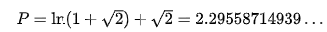
\includegraphics[width=8.65cm,height=0.85cm]{media/image1.png}
\end{figure}


The circle�and parabola are unique among conic sections 
in that they have a universal constant; the analogous ratios for
ellipses�and hyperbolas�depend on their
eccentricities. This means that all circles are
similar�and all parabolas are similar, whereas ellipses 
and hyperbolas are not.

\begin{figure}[h]
\centering
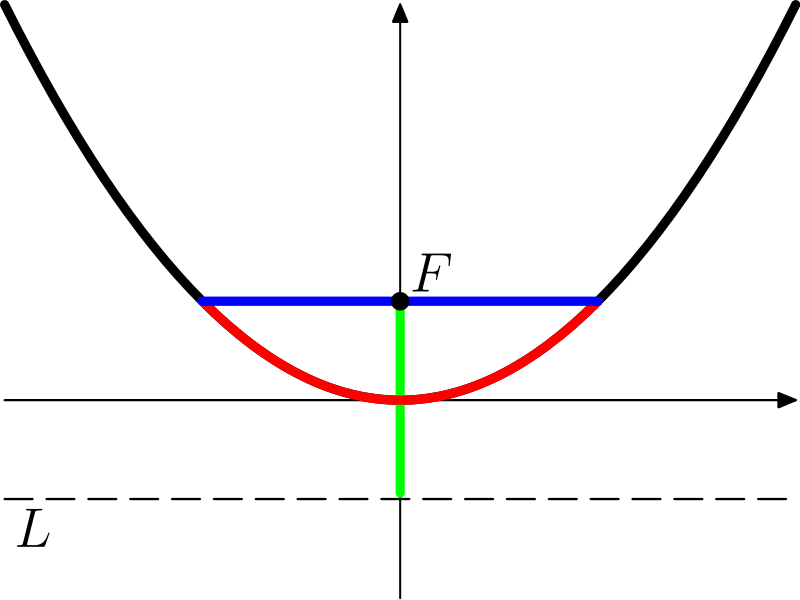
\includegraphics[width=10.16cm,height=7.62cm]{media/image2.png}
\end{figure}




Definitions - 

The \textbf{latus rectum}�of a conic section is the chord through a 
focus parallel to the conic section directrix (Coxeter 1969). "\textbf{
Latus rectum}" is a compound of the Latin\textbf{latus}, meaning 
"side," and\textbf{rectum}, meaning "straight." Half the\textbf{
latus rectum}�is called the semilatus\textbf{rectum}.

REFERENCES 

$[$1 Weisstein, Eric W.�"Latus Rectum." From\textit{MathWorld}--A 
Wolfram Web Resource.�http://mathworld.wolfram.com/LatusRectum.html









\end{document}
